\chapter{Protocol}
\label{chapter:protocol}
This chapter describes the low-level peer-to-peer protocol that runs Bitcoin.
Unfortunately, the Bitcoin protocol has never been documented properly:
the original paper \cite{bitcoin_2009} does not describe the details of the protocol and no official and complete description is available.
Some unofficial documentation does exist, but it is often incomplete and outdated.
The single point of truth available is the open-source original Bitcoin client, \texttt{bitcoind} \cite{bitcoin_github}:
at the time of writing, around \num{95}\% of nodes in the network run some version of this client \cite{bitnodes}.
Unfortunately, the source code is quite hard to understand and contains almost no comment.
The content of this chapter is thus primarily based on academical papers \cite{eclipse_attack_2015, deanonymization_2014}, on some online references \cite{bitcoin_reference, bitcoin_guide} and partially on the source code itself.
Please note that the content of this chapter refers to \texttt{bitcoind}:
other clients may choose different settings or strategies and behave slightly differently in some cases.

\medskip
Peers in the Bitcoin network are identified by their IP address.
Each node can initiate up \num{8} outgoing connections with other nodes, and accept up to \num{117} incoming connections, for a total of \num{125} \footnote{With the default settings (it is possible to configure custom values if necessary). Measures show that the majority of nodes have at most \num{8} outgoing connections and never reach the maximum number of incoming ones \cite{discovering_influential_nodes_2014}.}.
All connections use unencrypted TCP channels.
Nodes propagate and store only public IP addresses.
At the moment of writing, there are about \num{9000} reachable server, while the number of clients is estimated to be between \num{100000} and \num{200000}.
Nodes can also connect to the network via Tor \cite{bicoin_tor}.

\medskip
We divide the description of the protocol in \num{2} layers: topology and core.
Both layers use an epidemic (or gossip) paradigm \cite{gossip_1987} to achieve a fast information propagation and be tolerant to failures.


\section{Topology}
\label{sec:topology}
The topology layer is responsible to create and maintain the a peer-to-peer overlay network between Bitcoin nodes.
Its main functions are:
\begin{itemize}
	\item discover new peers in the Bitcoin network;
	\item propagate the IP addresses of nodes in the network;
	\item detect and remove peers that left the network or are offline for a long period of time;
	\item form an overlay network that can be used to efficiently broadcast blocks and transactions to all peers in the network (see \cref{sec:core});
	\item detect misbehaving peers and ban them if necessary.
\end{itemize}

\subsection{Peer discovery}
\label{sub:discovery}
The peer discovery phase is crucial for the bootstrap of the network:
at the first startup, a Bitcoin node does not know anything about the other peers.
Bitcoin nodes use different strategies to discover the first peers to connect to:
this allows to achieve a higher failure resistance and security, since an attacker might be able to interfere with some of the strategies, but it is less unlikely that it might interfere with all of them \cite{bitcoin_peer_discovery}.
Once a node connects to the first peer, it can start to run the Bitcoin protocol to gather information about other connected peers.

\subsubsection{IP discovery}
The first step in peer discovery is to get its own IP address.
After the startup, a Bitcoin node issues a HTTP GET request to \num{2} hard-coded websites, which reply with the IP address assigned by the \ac{ISP}:
the client reads the HTTP response and parses the IP address \cite{bitcoin_peer_discovery}.
It is possible that the node discovers more than one IP address:
in that case, public IP addresses are preferred over private ones \cite{deanonymisation_2014}.
When a client establishes an outgoing connection to a remote peer, it first sends a \texttt{Version} message to advertize the chosen address (see \cref{par:version}).

\subsubsection{Callback address}
When a node receives an incoming connection, the remote node sends a \texttt{Version} message containing its IP address.
After sending its own address, it sends a \texttt{GetAddr} request message to the remote node to learn about more addresses.

\subsubsection{DNS seeders}
A DNS seeder is a server that responds to \ac{DNS} queries from Bitcoin nodes with a list of IP addresses of other nodes.
The seeder obtains these addresses by periodically crawling the network, looking for active peers.
At the time of writing, the Bitcoin network has \num{7} seeder and their hosts are hard-coded in the client source code \cite{bitcoin_dns}:
each server is maintained by members of the Bitcoin community.
The number of addresses in the query response in limited by the \ac{DNS} constraints:
a typical \ac{DNS} packet over UDP contains up to \num{25} addresses \cite{dns_stackoverflow};
if used over TCP, a \ac{DNS} answer can contain up to \num{4000} addresses \cite{dns_4000}.
Please note that the list of addresses is not cryptographically-authenticated and could be easily compromised by an attacker with control of the victim's network (for example, mounting a man-in-the-middle attack) \cite{bitcoin_guide}.
The DNS seeders are queried only in the following \num{2} cases:
\begin{enumerate}
	\item a new node joins the network for the first time;
	\item an existing node restarts and fails to reconnect to the old peers; the seeders are queried only if the node has less than \num{2} outgoing connections and after \num{11} seconds since the initial connection attempt.
\end{enumerate}

\subsubsection{Addr messagges}
\texttt{Addr} messages are used to obtains network information from peers:
they contain up to \num{1000} IP addresses each \footnote{One \texttt{Addr} message can theoretically contain any number of addresses, however it is rejected by peers running recent versions of \texttt{bitcoind} is it contains more than \num{1000} addresses.} and can be either sent unsolicited or as a response to a particular event.
Addresses propagation using \texttt{Addr} message is discussed in details in \cref{sub:address-propagation}.

\subsubsection{Database of known addresses}
All peers discovered with various strategies are stored in a database of known IP addresses locally to the node.
When the node restarts, if can use the database to randomly select some nodes to connect to.
The idea is behind this strategy is that Bitcoin nodes can change IP address over time, but it is unlikely that all of them change address at the same time:
after a restart, the node is likely to be able to connect to some of the old peers.

\subsubsection{Hard-coded seed addresses}
The client contains hard coded IP addresses that represent bitcoin nodes:
at the moment, the list contains about \num{1250} IP addresses \cite{bitcoin_seeds}.
The list is regularly updated by the Bitcoin contributors, so that clients running the latest versions of \texttt{bitcoind} have good chances to find some Bitcoin nodes willing to accept incoming connections.
These addresses are only used as a last resort, if no other method has produced any address at all.

\subsubsection{Configuration}
Finally, a user can specify peer addresses in the software configuration, either with command line options or providing a text file of addresses.
These addresses are not advertized in response of a \texttt{GetAddr} message \cite{bitcoin_peer_discovery}.
The user can also specify the first peer to connect to.

\subsection{Address propagation}
\label{sub:address-propagation}
Bitcoin uses \texttt{Addr} messages to propagate information about peers in the network and construct the topology.
Each node maintains a list of addresses of other peers in the network:
each address is given a timestamp which determines it freshness.
A node can store up to \num{20480} addresses, stored in different tables:
the \texttt{tried} table contains addresses of peers to whom the node has successfully established a connection and is limited to \num{4096} addresses;
the \texttt{new} table contains addresses for peers to whom the node has not yet initiated a successful connection is limited to \num{16384} addresses.

\texttt{Addr} messages can be solicited or unsolicited.
Nodes can request list of known addresses from each other using a \texttt{GetAddr} message:
this is usually done only when a new outgoing connection is established (the protocol does not prevent a client from issuing a \texttt{GetAddr} message at any time) \cite{eclipse_attack_2015}.
When a node receives a \texttt{GetAddr} message, it sends back \num{23}\% of the number of addresses stored in the database (chosen randomly), but no more than \num{2500} in total \cite{deanonymisation_2014}.
If the number of addresses exceeds the limit of \num{2500}, multiple \texttt{Addr} messages are sent.

Nodes periodically push \texttt{Addr} messages to its peers:
each day, a node sends its own IP address in an \texttt{Addr} message to each peer it is connected to \cite{eclipse_attack_2015}.

Whenever a node receives an \texttt{Addr} message, it decides whether to forward it to its neighbors;
the decision is taken individually for each address in the messages.
An address is forwarded only if:
\begin{itemize}
	\item the total number of addresses in the corresponding \texttt{Addr} message does not exceed \num{10};
	\item the timestamp attacked to the address is not older than \num{10} minutes.
\end{itemize}
If both checks pass, the node schedules a new \texttt{Addr} message containing the address to \num{2} randomly chosen nodes \footnote{Actually, if the address is non-reachable for the node (e.g. the node supports only IPv4 and the address is IPv6) it is forwarded to only \num{1} peer.}.
The actual transmission of the scheduled \texttt{Addr} messages does not happen immediately.
The messages are divided in queues for different peers.
Every \num{100} milliseconds, the node randomly selects one of the queues and flushes all the present messages.
The node selected in the current round is the \textit{trickle node} \cite{deanonymisation_2014}; the whole procedure is called \textit{trickling} and is illustrated in \cref{fig:trickling}.
To prevent stale \texttt{Addr} messages from endlessly propagating, each Bitcoin node remembers the messages forwarded to each connected peer:
before forwarding an address, the node checks if the address was already sent over the same connection and avoids sending it again \cite{eclipse_attack_2015}.
The lists of messages are flushed daily.

\begin{figure}[ht!]
	\begin{subfigure}{.42\textwidth}
		\vspace*{0.25cm}
		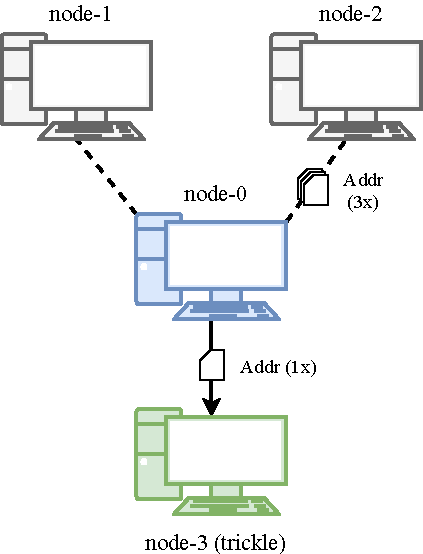
\includegraphics[width=\columnwidth]{figures/trickling_1}
		\vspace*{0.1cm}
		\caption{
			Round \num{1}:
			\texttt{node-3} is selected as trickle.
		}
		\vspace*{0.2cm}
	\end{subfigure}
	\hfill
	\begin{subfigure}{.42\textwidth}
		\vspace*{0.25cm}
		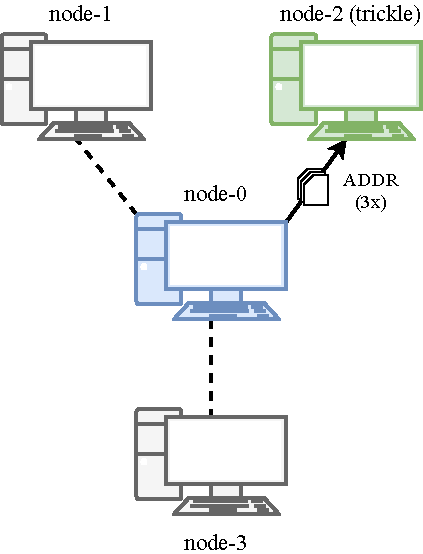
\includegraphics[width=\columnwidth]{figures/trickling_2}
		\vspace*{0.1cm}
		\caption{
			Round \num{2}:
			\texttt{node-2} is selected as trickle.
		}
		\vspace*{0.2cm}
	\end{subfigure}
	\caption[Illustration of the trickling procedure]{
		Illustration of the trickling procedure of \texttt{Addr} messages.
		\texttt{node-0} (in blue) gets an \texttt{Addr} message and select \texttt{node-3} and \texttt{node-2} for forwarding.
		An \texttt{Addr} message is added to the queues of both nodes, that count respectively \num{1} and \num{3} messages.
		\texttt{node-3} is chosen at round \num{1} and its queue is flushed:
		the scheduled \texttt{Addr} message is sent.
		\texttt{node-2} is chosen at round \num{2}:
		all \num{3} messages in queue are sent together to the destination.
	}
	\label{fig:trickling}
\end{figure}

\subsection{Peer cleanup}
\label{sub:peer-cleanup}
Bitcoin nodes exchange control messages to verify that remote peers are still connected and working correctly.
Every \num{2} minutes, each node sends a \texttt{Ping} message to all connected peers \cite{bitcoin_ping_pong}:
upon receiving a \texttt{Ping} message, the node immediately replies with a \texttt{Pong}.
If a node does not receive any \texttt{Pong} message from a peer for \num{20} minutes, it assumes the peer to be not working and drops the connection.

\subsection{Misbehaving peers}
Bitcoin implements a reputation-based protocol.
Each connection is associated with a penalty score:
whenever the node receives a malformed messages, it increases the penalty score for the sender;
if the score reaches a threshold, the IP address of the corresponding peer is banned for \num{24} hours \cite{deanonymisation_2014}.
This mechanism helps Bitcoin to detect and attenuate denial-of-service attacks.

\subsection{Control messages}
Bitcoin nodes exchange information in messages, sent over the persistent TCP connections.
Messages have a header and a body:
the header always contains a fixed start string that delimits the message start, the name of the command, the size of the body and a checksum;
the body changes depending on the specific message and can be empty in some cases.
None of the control messages are authenticated in any way:
they could potentially contain incorrect or intentionally harmful information.

\begin{figure}[ht]
	\centering
	\vspace*{0.25cm}
	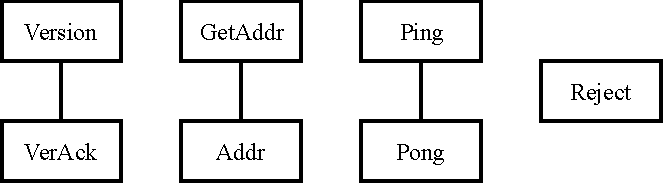
\includegraphics[scale=0.85]{figures/control_messages}
	\vspace*{0.25cm}
	\caption[Overview of the Bitcoin control messages]{
		Overview of the Bitcoin control messages:
		lines between boxes indicate that the corresponding messages are correlated.
	}
	\label{fig:control-messages}
\end{figure}

Some messages are related to each other \cite{bitcoin_reference}, as illustrated in \cref{fig:control-messages}:
one is usually the reply to the other (for example, \texttt{Version} and \texttt{VerAck});
in some cases, one message can be both the reply of another one and be used alone (for example, \texttt{Addr}).
Many of the control messages have been touched already in the description of the protocol:
this section gives an overview of the main ones.

\subsubsection{Version}
\label{par:version}
The \texttt{Version} message provides information to the receiving node about the node that initialized an outgoing connection.
If the incoming connection is accepted, the receiving node should reply with a \texttt{VerAck} message before sending any other message through that channel.
Until both peers have exchanged the \texttt{Version} and \texttt{VerAck} messages, no other messages will be accepted.
The \texttt{Version} message also contains information about the client version, user-agent, configuration, sender and receiver IP addresses.

\subsubsection{VerAck}
The \texttt{VerAck} message acknowledges a previously received \texttt{Version} message and accepts the incoming connections:
it informs the connecting node that it can begin to send other messages.
The \texttt{VerAck} message has no payload and is sent only in reply to a \texttt{Version} message.

\subsubsection{GetAddr}
The \texttt{GetAddr} message requests an \texttt{Addr} message containing IP addresses of other nodes in the network from the receiving node.
The transmitting node can use the message to quickly update its list of available nodes, rather than waiting for unsolicited \texttt{Addr} messages.
The \texttt{GetAddr} is usually sent on new outgoing connections after receiving the \texttt{VerAck} from the other peer.
The \texttt{GetAddr} message has no payload.

\subsubsection{Addr}
The \texttt{Addr} messages relays information about other known peers in the network (IP address and TCP port).
The message can contain up to \num{1000} items:
if a node wants to transmit information about more than \num{1000} peers, it need to send multiple \texttt{Addr} messages.
An \texttt{Addr} can be sent in reply to a \texttt{GetAddr} message or unsolicited (daily to broadcast the node's self IP address, or to forward a newly received address):
details about the situations in which an \texttt{Addr} message is sent are discussed in \cref{sub:address-propagation}.

\subsubsection{Ping}
The \texttt{Ping} message helps the transmitting node to verify that the receiving peer is still connected.
If a networking error at either the TCP or IP level is encountered when sending the \texttt{Ping} message (e.g. a connection timeout), the transmitting node can assume that the receiving node is disconnected.
The response to a \texttt{Ping} message is the \texttt{Pong} message.
The \texttt{Ping} message contains a nonce in the payload that needs to be included in the reply \texttt{Pong} message:
this allows nodes to keep track of the latency.

\subsubsection{Pong}
The \texttt{Pong} message is sent as a reply to a previously received \texttt{Ping} message:
it confirms that the current node is alive and correctly connected to the node that sent the \texttt{Ping} message.
The \texttt{Pong} message include the nonce sent in the original \texttt{Ping} message.

\subsubsection{Reject}
The \texttt{Reject} message informs the receiving node that one of its previous messages has been rejected.
The message contains information about the rejected message and the reason for that.
Examples of rejection reasons are a malformed block or a peer running an obsolete version of the protocol.


\section{Core}
\label{sec:core}
The core layer uses the underlying overlay network created by the topology layer to propagate blocks and transactions to all Bitcoin nodes.
Its main functions are:
\begin{itemize}
	\item quickly propagate transactions to a big portion of the network, so they can be included in some block in a short time;
	\item propagate blocks as fast as possible to minimize the work wasted on orphan blocks.
\end{itemize}

\subsection{Transaction propagation}
Transactions are propagated using \texttt{Tx} messages:
when a client generates a new transaction, it packages it in a \texttt{Tx} message and relays it to some Bitcoin node \cite{bitcoin_reference}.
Similarly to \texttt{Addr} messages, \texttt{Tx} messages are not always immediately forwarded to all peers \cite{deanonymisation_2014}:
there are immediately sent with a probability of \num{0.25};
otherwise, they are put in the queue of the corresponding peer and flushed with the peer becomes the trickle node (see \cref{sub:address-propagation}).

The transaction is then propagated to the entire network.
Forwarding a transaction from one peer to another involves several steps:
\begin{itemize}
	\item the sender node transmits an \texttt{Inv} message of type ``transaction'' containing the hash of the new transactions;
	\item the receiver checks if it knows already the hashes; if it is the case, no further step is performed;
	\item if the hashes are new, the receiver sends a \texttt{GetData} message to request the transmission of the full transactions;
	\item the sender transmits one \texttt{Tx} message for each requested transaction;
	\item when the receiver gets the transactions, it advertizes them to its peers with an \texttt{Inv} message.
\end{itemize}

As with \texttt{Addr} messages, each Bitcoin node maintains a list of forwarded transactions for each peer and avoids to forward the same transaction to the same peer twice.
Each node keeps the list of all received transactions in its memory pool.
If it receives a transaction with the same hash as one in the pool or in a block in the main chain, the received transaction is rejected.
Each node also keeps track of the transactions already included in the main chain and avoids to include them in new blocks.
On the other hand, if a block is orphaned, the transactions which are not already in another block on the main chain are again available for the next blocks.

\subsection{Block propagation}
Blocks are propagated in a similar way as transactions.
When a new block is generated, the miner sends a \texttt{Block} message to all its peers.
When a node receives a block, it checks its validity and then forwards it to all connected peers.
To avoid broadcasting the block too many times, nodes maintain a list of already sent blocks:
each time they receive a block, they first check if that block was already forwarded;
only if the answer is negative, the node sends it to its peers.

\medskip
Blocks can also be requested an need with a \texttt{GetBlock} message:
this mechanism is used when a node receives a block with an unknown parent (in case \num{2} subsequent blocks are mined, it is possible for some nodes in the network to receives the second before the first one), or for the bootstrap of a new node, as explained in the next section.

\subsection{Initial block download}
New miners do not have any information about the current status of the blockchain.
Once they successfully connect to some peers in the network, they need to download the entire blockchain to be able to verify the new transactions and mine new blocks.
This procedure is called \textit{initial block download} and works as follows:
\begin{itemize}
	\item the new miner selects one of the connected peers, called the \textit{sync node}, and sends it a \texttt{GetBlocks} message, requesting all blocks after the genesis (the only known block, since it is hard-coded in the software);
	\item upon receipt of the \texttt{GetBlocks} message, the sync node searches its local longest chain, starting from the genesis; it then replies with an \texttt{Inv} message containing the hashes for the first \num{500} blocks after the genesis (the maximum allowed for a single response);
	\item the miner replies with a \texttt{GetData} message and requires the transmission of the complete missing blocks;
	\item upon receipt of the \texttt{GetData} message, the sync node replies with a \texttt{Block} message for each requested block;
	\item the miner validated each received blocks; the miner then sends a new \texttt{GetBlocks} message to request the next blocks;
	\item the process is repeated until all blocks in the longest chain has been transmitted.
\end{itemize}
The same procedure can be used if a miner goes offline for some period of time and wants to fast get up-to-date with the current state of the blockchain.

\subsection{Data messages}
Similarly to the control messages, data messages have header and body, and are sometimes correlated to each other.
Serialized messages and are not authenticated in any way, but both transactions and blocks can be easily verified:
a transaction is valid only if correctly signed with the private key of the sender address, while blocks are valid only if their hash is less or equal to the current target.

\medskip
\cref{fig:data-messages} illustrates the main data messages used by the core layer of the Bitcoin protocol;
each message in explained in detail in a dedicated section.

\begin{figure}[ht]
	\centering
	\vspace*{0.25cm}
	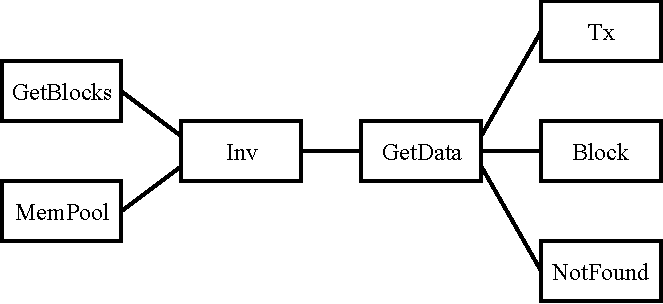
\includegraphics[scale=0.85]{figures/data_messages}
	\vspace*{0.25cm}
	\caption[Overview of the Bitcoin data messages]{
		Overview of the Bitcoin data messages:
		lines between boxes indicate that the corresponding messages are correlated.
	}
	\label{fig:data-messages}
\end{figure}

\subsubsection{GetBlocks}
The \texttt{GetBlocks} message requests an \texttt{Inv} message that provides the hashes of blocks starting from a particular point in the block chain.
It allows a peer which has just joined the network for the first time or has been disconnected or started for a while to get information about the current state of the blockchain and later request unseen blocks.
Note that the receiving peer may respond with an \texttt{Inv} message containing hashed of orphaned blocks:
it is responsibility of the requesting node to poll all its peers to find the longest chain.

\subsubsection{MemPool}
The \texttt{MemPool} message requests the hashes of valid transactions that has not yet been stored in a block in the longest chain.
That is, transactions which are in the receiving node’s memory pool.
The response to the \texttt{MemPool} message are one or more \texttt{Inv} messages containing the hashes of all transactions in the memory pool.
The message is particularly useful for new miners that just joined the network to get quickly up-to-date with the list of transactions available for the next block.
It is also used by non-miner clients that quickly want to check the state of a new transaction just submitted to the network.
The \texttt{MemPool} message has no body.

\subsubsection{Inv}
The \texttt{Inv} message transmits one or more inventories (hashes, used as unique identifiers) of objects (blocks or transactions) known to the transmitting peer.
It can be sent unsolicited to announce new transactions or blocks, or it can be the reply to a \texttt{GetBlocks} message or \texttt{MemPool} message.
The receiving peer can compare the inventories contained in an \texttt{Inv} message to determine the unseen object and require them using a \texttt{GetData} message.
An \texttt{Inv} message must contain all objects of the same type.

\subsubsection{GetData}
The \texttt{GetData} message requests one or more objects from another node.
The objects are requested by their hashes (inventories), which the requesting node usually discovers from \texttt{Inv} messages.
The response to a \texttt{GetData} message depends on the requested object and can be a \texttt{Tx} message, \texttt{Block} message, a \texttt{NotFound} message, or other special messages not described in this text.

\subsubsection{Tx}
The \texttt{Tx} message transmits a single transaction.
It can be sent either unsolicited, for new transactions generated by the node, or in response to a \texttt{GetData} message.
The body of a \texttt{Tx} message contains a single serialized transaction.

\subsubsection{Block}
The \texttt{Block} message transmits a single block.
It can be sent for \num{2} different reasons:
\begin{enumerate}
	\item solicited, in response to a \texttt{GetData} message that requests block objects;
	\item unsolicited, broadcasting a newly-mined blocks to all of nodes in the network.
\end{enumerate}

\subsubsection{NotFound}
The \texttt{NotFound} message is a reply to a \texttt{GetData} message which requested an object unknown or not available to relay (for example, Bitcoin nodes does not need to relay historic transactions that are already been included in the blockchain).
The body includes the hashes of object that were not found on the receiving node.
